\chapter{\IfLanguageName{dutch}{Proof of concept}{Proof of concept}}%
\label{ch:proofofconcept}

Dit hoofdstuk beschrijft eerst welke technologieën gebruikt zijn voor het ontwikkelen van ``Move-it!''. Daarna wordt de opbouw van de webapplicatie besproken en geïllustreerd met schermafbeeldingen. Daarbij wordt ook telkens geduid welke gamificationtechnieken gebruikt zijn.

\section{Gekozen technologieën}

\subsection{Framework}

Gezien de expertise van \href{https://www.we-are.be/}{we are}, is er voor het platform gekozen voor een responsive React\footnote{\href{https://react.dev/}{https://react.dev/}}-website. React is een gratis en open source JavaScript library, die gebruikt wordt voor het ontwikkelen van gebruikersinterfaces door middel van componenten. In plaats van JavaScript, is er voor dit project echter gebruik gemaakt van TypeScript \footnote{\href{https://www.typescriptlang.org/}{https://www.typescriptlang.org/}}. TypeScript is een object-georiënteerde programmeertaal, ontwikkeld door Microsoft Corporation. Er is voor TypeScript gekozen wegens diens type-safety. Dit wil zeggen dat type-errors vroeger in het ontwikkelproces opgevangen kunnen worden, wat de ontwikkeltijd bevordert.

Voor de implementatie van authenticatie is er gebruik gemaakt van Auth0\footnote{\href{https://auth0.com/}{https://auth0.com/}}. De redenen waarom er voor Auth0 gekozen is, zijn: de mogelijkheid om aan te melden met een Google-account, efficiënte integratie in React en de mogelijkheid tot een gratis abonnement wanneer het aantal gebruikers onder de 7000 blijft, wat voor deze POC meer dan voldoende is.

\subsection{Component libraries}
Een component library is een set van voorgedefinieerde, geteste en gedocumenteerde ``User Interface'' (UI) componenten, die makkelijk hergebruikt kunnen worden over een hele applicatie\footnote{\href{https://www.uxpin.com/studio/blog/ui-component-library/}{https://www.uxpin.com/studio/blog/ui-component-library/}}.
De Material UI Core\footnote{\href{https://mui.com/core/}{https://mui.com/core/}} en Material UI X\footnote{\href{https://mui.com/x/}{https://mui.com/x/}} component libraries zijn gebruikt voor de ontwikkeling van deze website. Er is gekozen voor Material UI wegens diens universele look-and-feel, het ruime aanbod aan gratis componenten en de beschikbaarheid van verschillende grafiek-componenten. Daarnaast zijn deze componenten uitermate geschikt voor zowel mobiel als desktop gebruik, wat de ``User Experience'' (UX) verbetert.

\subsection{Databank}

Een databank is een grote verzameling van gegevens. Een "Database Management System" (DBMS) is een systeem waarmee op een georganiseerde manier data beheerd, opgeslagen en opgevraagd kan worden.

Datbanken kunnen onderverdeeld worden in twee grote categorieën: relationele en niet-relationele databanken.

\subsubsection{Relationele databanken}

Relationele databanken slaan gegevens op aan de hand van tabellen die beschreven staan in een relationeel model \autocite{Elsabagh2022}.
De betrouwbaarheid van een  relationele databank wordt getoetst met ACID eigenschappen. Deze eigenschappen worden als volgt gedefinieerd door \textcite{Jatana2012}:

\begin{itemize}
    \item \textbf{Atomiciteit}: elke transactie die uitgevoerd wordt, wordt als een ondeelbare eenheid beschouwd. Dit wil zeggen dat een transactie oftewel helemaal, oftewel helemaal niet uitgevoerd wordt.
    \item \textbf{Consistentie}: dit garandeert dat een databank zich voor en na elke transactie in een consistente staat bevindt.
    \item \textbf{Isolatie}: dit zorgt er voor dat transacties onafhankelijk van elkaar worden uitgevoerd. Dit wil zeggen dat concurrerende transacties, die bijvoorbeeld op dezelfde data bewerkingen uitvoeren, na elkaar uitgevoerd worden.
    \item \textbf{Duurzaamheid}: nadat een transactie gecommit is, zal deze permament in de databank opgeslagen worden, zelfs in het geval van bijvoorbeeld een systeemcrash of het uitvallen van de stroom.
\end{itemize}

\subsubsection{Niet-relationele databanken}
Niet-relationele databanken daarentegen zijn schemaloos en kunnen zeer grote hoeveelheden data bevatten. Daarnaast wijken dit type databanken ook af van de ACID- eigenschappen, in die zin dat ze slechts eventuele consistentie kunnen garanderen \autocite{Elsabagh2022}. Enkele theoretische begrippen bij niet-relationele databanken zijn: BASE en CAP.

BASE staat volgens \textcite{GaneshChandra2015} voor:

\begin{itemize}
    \item \textbf{Basically Available}: de databank is altijd beschikbaar, omdat dit type databank meerdere kopieën van de data op meerdere fysieke plaatsen bewaart.
    \item \textbf{Soft state}: de staat van de databank kan veranderen over de tijd heen.
    \item \textbf{Eventual consistency}: de databank zal uiteindelijk consistent worden, maar kan in tussentijd wel inconsistent zijn.
\end{itemize}

Het CAP-theorema werd voor de eerste keer voorgesteld in 2009 door \textcite{Simon2012}. Dit theorema stelt dat het voor een gedistribueerd systeem zeer moeilijk is om tegelijkertijd zowel consistent, beschikbaar als partitie tolerant te zijn. Dit wil zeggen dat een systeem slechts aan één van de twee eigenschappen kan voldoen \autocite{Elsabagh2022}.

De meest voorkomende types van niet-relationele databanken zijn document-, kolom- en graafdatabanken en key-value stores \autocite{Elsabagh2022}.

\begin{itemize}
    \item \textbf{Document-databanken}: dit type databank slaat documenten op in JSON-formaat. Volgens \textcite{Sullivan2015} zijn document-databanken het meest voorkomende type niet-relationele databank.
    \item \textbf{Kolom-databanken}: dit type databank slaat data op in kolommen in plaats van in rijen. Dit wil zeggen dat de gegevens van eenzelfde eigenschap bij elkaar opgeslagen wordt. Op kolom-databanken kunnen geen JOIN-operaties uitgevoerd worden \autocite{Sullivan2015}.
    \item \textbf{Graafdatabanken}: volgens \textcite{Elsabagh2022} zijn graafdatabanken de toekomst van databanken. Om data op te slaan, worden vertices (ook wel nodes genoemd) en edges (ook wel relaties genoemd) gebruikt. Zowel nodes en relaties kunnen attributen bevatten.
    \item \textbf{Key-value stores}: dit is de simpelste vorm van niet-relationele databanken. Data wordt er opgeslagen in key-value paren, waarbij de key een unieke waarde is waarmee de value opgevraagd kan worden. Deze value kan eender welke datastructuur hebben: bijvoorbeeld een string, een integer of zelfs een afbeelding.
\end{itemize}

\subsubsection{Keuze van de databank}

Deze applicatie gebruikt een graafdatabank, meer specifiek Neo4J\footnote{\href{https://neo4j.com/}{https://neo4j.com/}}.

Er is in deze situatie gekozen voor een graafdatabank omdat er, zoals net beschreven, dan geen databank-schema ontworpen moet worden, wat er voor zorgt dat het mogelijk is om snel te ontwikkelen en gaandeweg eventueel zaken aan te passen indien nodig.

Daarnaast zal de analyse van de ingegeven sportdata ook efficiënter verlopen. Door het gebruik van nodes en vertices zullen er geen complexe join-operaties aan te pas komen om bijvoorbeeld alle activiteiten van de deelnemers van een team op te vragen, wat bij een relationele databank wel het geval zou zijn. Dit komt de kwaliteit van de analyse ten goede.

\subsection{Deployment}

De website wordt gedeployed met behulp van Vercel, die een frontend-as-a-service product aanbiedt\footnote{\href{https://vercel.com/home}{https://vercel.com/home}}. De GitHub\footnote{\href{https://github.com/}{https://github.com/}}-repository van deze applicatie is gelinkt aan een Vercel-project, wat er voor zorgt dat elke nieuwe commit op de main-branch steeds gedeployed zal worden. Dit maakt het zeer beheersvriendelijk.

``Move-it!'' is terug te vinden op \href{https://move-it-ghent.vercel.app/}{https://move-it-ghent.vercel.app/}.

\section{Opbouw van de applicatie en geïntegreerde gamificationtechnieken}

De applicatie is opgesteld uit twee basis bouwstenen: een navigatiemenu bovenaan, en een centrale pagina. Afhankelijk van de gekozen navigatie, zal deze centrale pagina een dashboard, een overzicht van eigen prestaties, een oplijsting van de teamleden of een profielpagina vertonen.

Er is tijdens de ontwikkelingsfase ook aandacht besteed aan mobiele gebruikers, zo zal de webapplicatie mee schalen wanneer deze van op een kleiner scherm opgeroepen wordt.

\subsection{Dashboard}
Op het dashboard is de meeste informatie te zien: zowel de persoonlijke evolutie over één week en het overzicht van de types van de uitgevoerde activiteiten van de ingelogde gebruiker (zie figuur \ref{fig:graphs}), als de team en persoonlijke rankings (zie figuur \ref{fig:personalRanking} en \ref{fig:teamRanking}) zijn er te vinden. Dit is het centrale punt voor de toepassing van gamificationtechnieken.

De persoonlijke vooruitgang wordt namelijk in een grafiek weergegeven, waardoor een gebruiker gestimuleerd kan worden om zichzelf steeds te proberen overtreffen. \linebreak \textcite{Schiewe2020} hebben namelijk aangetoond dat de visualisatie van sportdata sporters op meerdere vlakken ten goede komt, waaronder hun motivatie. Dit kan mee verklaard worden door de motivatietheorie van \textcite{Siang2003} (zie \ref{ssec:werking-gamification}), waarbij op het zesde niveau van de hiërarchische behoeftepiramide voor gamers het belang van goede graphics wordt benadrukt. Uiteraard valt af te wachten of deze keuze op basis van de literatuur ook bevestigd kan worden voor sedentaire beroepen.

Bij de team en persoonlijke rankings worden de punten in de vorm van gepresteerde uren weergegeven. Om kleinere teams evenveel kans te geven, houdt de teamranking rekening met de grootte van het team bij de berekening. Concreet wil dit zeggen dat het gemiddeld aantal minuten beweging per gebruiker wordt gebruikt voor deze ranking, in plaats van de absolute som van de gepresteerde minuten van alle gebruikers van een team. Op die manier blijft een eerlijke competitie behouden, wat volgens \textcite{Ivanova2019} de motivatie verhoogt. Een logisch gevolg van de “Self-determination theory” van \textcite{Deci1985}, die stellen dat het gevoel van competentie één van de drie fundamenten voor motivatie is, en via de speldynamiek “competitieve elementen” kan worden opgewekt \autocite{Kam2018}.

\begin{figure}[h]
    \caption[Team ranking]{De team ranking, gezien vanop een laptop.}
    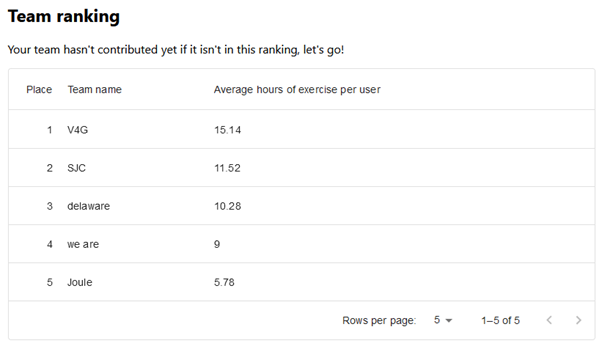
\includegraphics[width=1\textwidth]{TeamRanking}
    \label{fig:teamRanking}
\end{figure}

\begin{figure}[h]
    \caption[Persoonlijke ranking]{De persoonlijke ranking, gezien vanop een laptop. De achternamen van de gebruikers zijn onherkenbaar gemaakt om privacy-redenen.}
    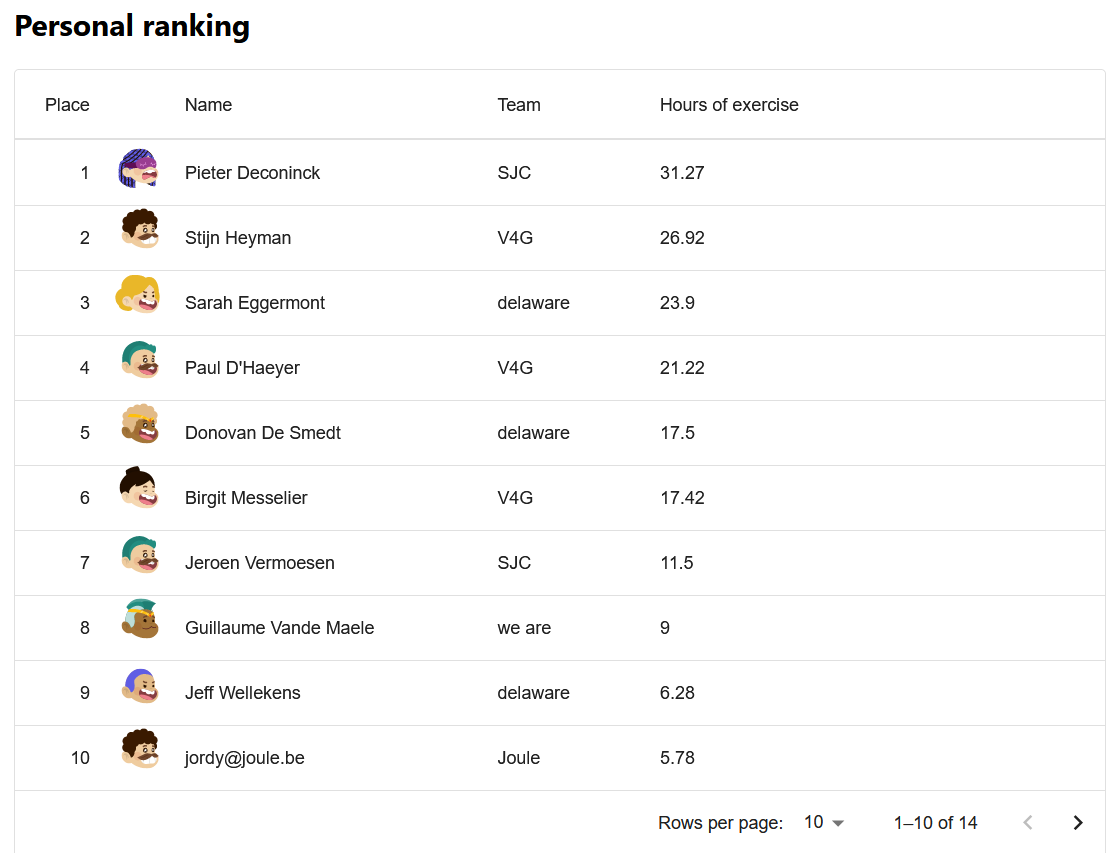
\includegraphics[width=1\textwidth]{PersonalRanking}
    \label{fig:personalRanking}
\end{figure}

Samengevat, is op het dashboard wat betreft gamificationtechnieken vooral ingezet op het creëren van een onderlinge competitie en het visualiseren van persoonlijke vooruitgang om zo de intrinsieke motivatie te proberen verbeteren, door middel van de scoreborden en de grafieken.

\begin{figure}[h]
    \caption[Overzicht prestaties dashboard website]{Overzicht van gepresteerde uren de afgelopen week en van het type activiteiten sinds de lancering van de applicatie, gezien vanop een laptop.}
    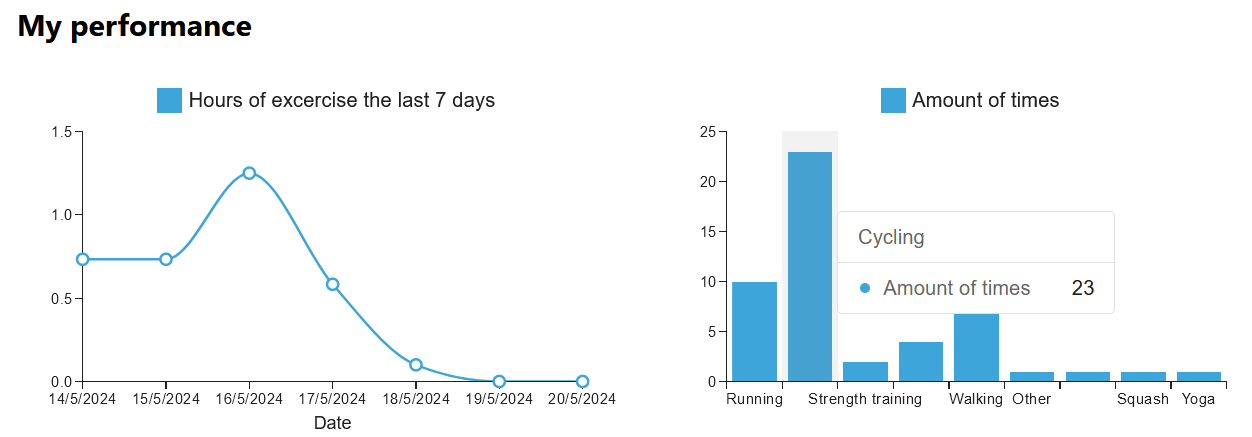
\includegraphics[width=1\textwidth]{MyGraphs}
    \label{fig:graphs}
\end{figure}

\subsection{Persoonlijk overzicht}
Op het persoonlijk overzicht is een lijst van de eigen gepresteerde activiteiten te zien (zie figuur \ref{fig:performances} en figuur \ref{fig:performancesMobile}), en kunnen gebruikers ook hun prestaties ingeven. Hier is voldoende ruimte voorzien voor het invullen van technische gegevens, zoals de gemiddelde hartslag en hoogtemeters. Afhankelijk van het type activiteit, en wanneer een afstand en duur ingegeven zijn, berekent de applicatie ook een gemiddelde snelheid. Zo kunnen frequente sporters een eventuele vooruitgang opmerken, wat ook motiverend kan werken.

\begin{figure}[h]
    \caption[Overzicht activiteiten website]{Overzicht van gepresteerde activiteiten in de applicatie, gezien vanop een laptop.}
    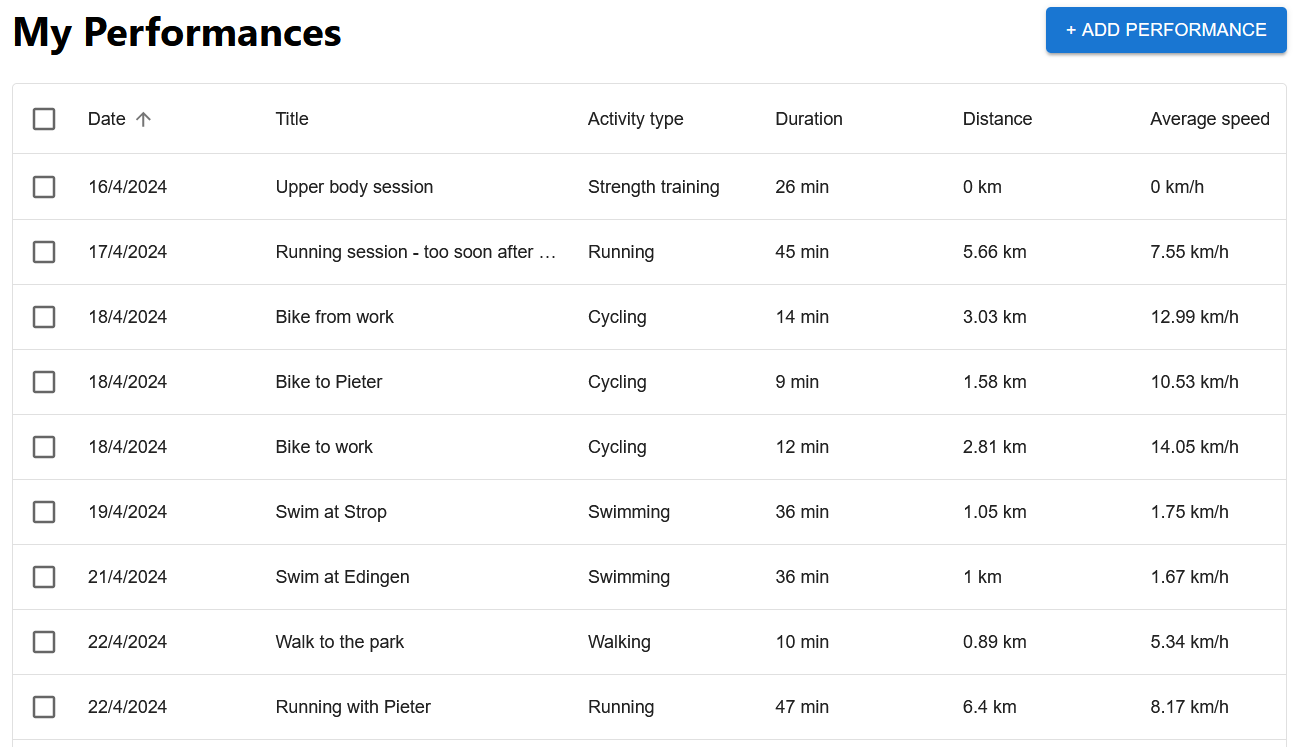
\includegraphics[width=1\textwidth]{MyPerformances}
    \label{fig:performances}
\end{figure}

\begin{figure}[h]
    \caption[Overzicht activiteiten website smartphone]{Overzicht van gepresteerde activiteiten in de applicatie, gezien vanop een smartphone.}
    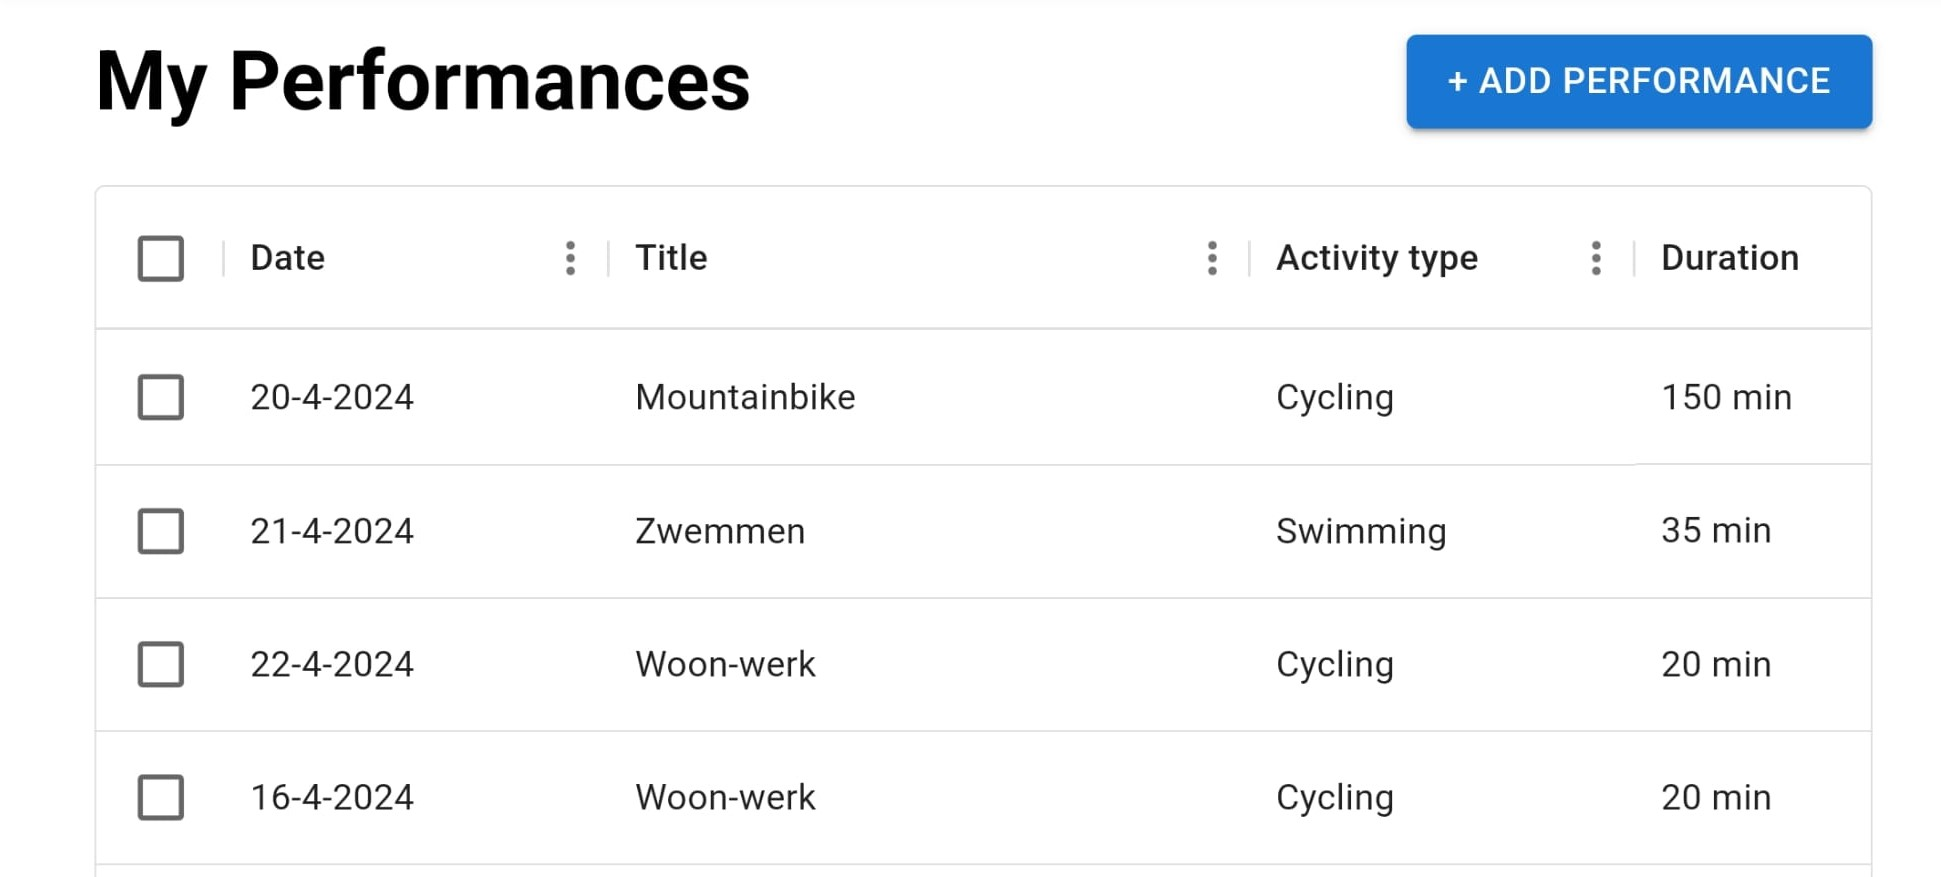
\includegraphics[width=1\textwidth]{MyPerformancesMobile}
    \label{fig:performancesMobile}
\end{figure}

\subsection{Teamoverzicht}

Dit overzicht is een oplijsting van alle teamleden waartoe de aangemelde gebruiker behoort (zie figuur \ref{fig:team}). Hiermee speelt het ontwikkelde sportplatform in op de bevindingen van \textcite{Kam2018}, die stelden dat via het opzetten van teams de verwantschap en verbondenheid behoefte uit de “Self-determination theory” kan worden vervuld  (zie \ref{ssec:werking-gamification}). Dat is een belangrijke voorwaarde om één van de meest besproken psychologische aspecten van gamification, motivatie, te genereren. Daarbij wordt motivatie gezien als de mediator voor het doelgedrag.

Om dit in de toekomst nog te versterken, zou ook de mogelijkheid toegevoegd kunnen worden om vanuit de applicatie andere mensen uit te nodigen. Zo kunnen reeds deelnemende gebruikers ook hun collega's, vrienden en/of familie uitnodigen.

\begin{figure}[h]
    \caption[Overzicht van teamleden]{Overzicht van teamleden in de applicatie, gezien vanop een laptop. Mailadressen zijn onherkenbaar gemaakt om privacy-redenen.}
    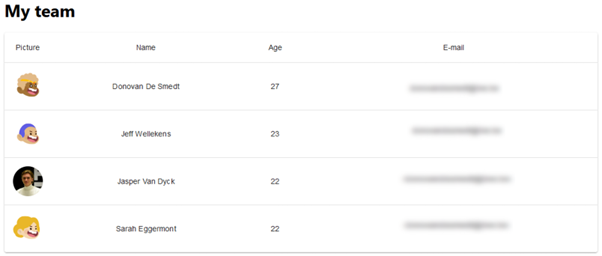
\includegraphics[width=1\textwidth]{MyTeam}
    \label{fig:team}
\end{figure}

\subsection{Profiel pagina}

Op deze pagina kan een gebruiker een avatar en naam kiezen waarmee die weergegeven wordt. Daarnaast moet een gebruiker bij de eerste aanmelding ook een team kiezen.